\chapter{Implémentation du moteur de jeu}

\section{Structures de données}
Le moteur de jeu est construit autour de trois classes :
\begin{itemize}
	\item \pyth{Tetramino} : les blocs 
	\item \pyth{Board} : la grille de jeu
	\item \pyth{TetrisEngine} : le moteur de jeu qui fait le lien entre les deux classes précédentes
\end{itemize} 

%Notons que toutes ces classes implémentent une méthode \pyth{copy(self)} qui envoie une copie de l'objet en utilisant le module \pyth{deepcopy}. 

%\section{La classe Tetramino}
%La classe \pyth{Tetramino} est responsable de le gestion des blocs et de leurs rotations. Elle est implémentée dans le fichier \pyth{tetramino.py}.

%Un bloc est défini par :
%\begin{itemize}
%	\item Un id, \pyth{self.id}, qui permet d'identifier son type.
%	\item Un glyphe de base, \pyth{self.base\_glyph}, qui représente la pièce sans rotation dans une matrice carrée. Chaque case occupée par le bloc est codée par son \pyth{id} et les cases vides par 0.
%	\item Le nombre de rotations possibles de la pièce, \pyth{self.nb\_rotations} (par exemple le O n'a qu'une seul rotation, le I en a deux et le T en a quatre).
%\end{itemize}
%
%Les rotations sont crées par la méthode \pyth{makeRotations(self)} au moment de la construction de la pièce  et sont stockées dans une liste de glyphs, \pyth{self.rotations}.\\ 
%Pour gérer les rotations, on utilise un attribut \pyth{self.glyph\_index} qui donne l'indice de la rotation courante, ainsi que le glyph courant, \pyth{self.glyph}.\\
%Enfin Deux méthodes permettent de faire tourner la pièce :
%\begin{itemize}
%	\item \pyth{rotate(self, direction='H')} : met à jour le glyph avec celui de sa rotation dans le sens donné (\pyth{'H'} pour le sens horaire et \pyth{'T'} pour le sens trigonométrique).
%	\item \pyth{setRotation(self, i)} : tourne directement la pièce dans la rotation d'indice \pyth{i}.
%\end{itemize}
%
%Notons également la méthode \pyth{getBoundingBox(self)} qui renvoie les coordonnées des coins des cases de la pièce réellement utilisées.
%
%Cette classe admet enfin quelques méthodes utiles :
%\begin{itemize}
%	\item \pyth{copy(self)} : renvoie une copie du bloc
%	\item \pyth{\_\_str\_\_(self)} : renvoie une chaîne de caractères pour afficher la pièce à des fin de test uniquement ici.
%\end{itemize}
%
%\medskip
%
%Dans ce fichier on définit également les pièces qui vont être utilisées, ainsi que la liste \pyth{BLOCK\_BAG} de toutes ces pièces.

\section{La classe Tetramino}
La classe \pyth{Tetramino} est responsable de le gestion des blocs et de leurs rotations. Elle est implémentée dans le fichier \pyth{tetramino.py}.

\subsection{Initialisation}
La représentation d'un bloc est codée par la liste des coordonnées de ses cases occupées, le coin en haut à gauche ayant pour coordonnées \pyth{(0,0)} :\\
Par exemple, pour le bloc "J" placé horizontalement :

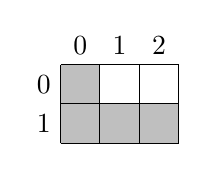
\begin{tikzpicture}[scale=0.5]
	\fill[color=lightgray] (0,0) rectangle (3,1);
	\fill[color=lightgray] (0,0) rectangle (1,2);
	\draw (0,0)--(3,0);
	\draw (0,1)--(3,1);
	\draw (0,2)--(3,2);
	\draw (0,0)--(0,2);
	\draw (1,0)--(1,2);
	\draw (2,0)--(2,2);
	\draw (3,0)--(3,2);
	
	\draw (0.5, 2) node[above]{0};
	\draw (1.5, 2) node[above]{1};
	\draw (2.5, 2) node[above]{2};
	\draw (0, 0.5) node[left]{1};
	\draw (0, 1.5) node[left]{0};
	
\end{tikzpicture}

Ce bloc sera codé par la liste \pyth{[(0,0), (1,0), (1,1), (1,2)]}\\

Lors de l'initialisation d'un bloc, on va donner :
\begin{itemize}
	\item Son \pyth{id} qui permettra d'identifier son type si besoin
	\item La liste de ses rotation dans le codage précédent
	\item Les coordonnées de son coin supérieur gauche et de son coin inférieur droit afin d'accélérer les tests de positionnement ultérieurs
\end{itemize}

\subsection{Rotations}
La rotation courante du bloc est mémorisée dans un attribut \pyth{glyph\_index} qui correspond à l'indice courant dans la liste de ses rotations.\\
On peut donner l'ordre :
\begin{itemize}
	\item Soit de tourner le bloc dans un sens avec la méthode \pyth{rotate(self, direction)}, où \pyth{direction} vaut \pyth{'H'} pour le sens horaire et \pyth{'T'} pour le sens trigonométrique.
	\item Soit de le placer directement dans une rotation désirée avec la méthode \pyth{setDirection(self, i)} où \pyth{i} est l'indice de la rotation voulue.
\end{itemize}

\subsection{Méthodes utilitaires}
Cette classe implémente une méthode \pyth{copy(self)} qui renvoie une copie du bloc ainsi qu'une méthode \pyth{toArray(self)} pour avoir une représentation matricielle dans une matrice carrée dans laquelle chaque case occupée vaut \pyth{id} et les case vides 0. Cette dernière méthode sera utile pour la pratie réseaux de neurones pour entrer la pièce sous la forme d'un vecteur 0/1. 

\subsection{Sacs de pièces}
Après la définition de la classe \pyth{Tetramino} on définit les constantes correspondant à chaque bloc et on en fait la liste dans des constantes \pyth{BLOCK\_BAG}.\\
Pour le moment il y a deux sacs de pièces :
\begin{itemize}
	\item \pyth{RAPID\_BLOCK\_BAG} : Chaque bloc a un nombre limité de rotation suivant ses symétries. Par exemple le bloc "I" n'a que deux rotations. Ce sac est utile pour les placements directs des pièces et économise des calculs inutiles.
	\item \pyth{CLASSIC\_BLOCK\_BAG} : Chaque bloc (sauf le "O") a quatre rotations pour coller aux règles du Tétris dans lesquelles un bloc tourne autour du centre de sa matrice carrée. Ce sac sera utile pour simuler le comportement d'un vrai joueur humain.	
\end{itemize}

\section{La classe Board}
La classe \pyth{Board} implémente la grille, ses méthodes de gestion (mise à jour des cellules, traitement des lignes,...) ainsi que les outils statistiques (nombre de trous, hauteur maximum,...). Elle est implémentée dans le fichier \pyth{board.py}.

\subsection{Constructeur}
Le constructeur de la classe \pyth{board} admet deux paramètres :
\begin{itemize}
	\item Sa largeur : \pyth{width}
	\item Sa hauteur : \pyth{height}
\end{itemize}

La grille en elle-même est stockée dans la liste double \pyth{self.grid} qui a pour largeur \pyth{width} et pour hauteur \pyth{height+2} (avec les deux lignes invisibles du dessus).

Enfin, les différents indicateurs statistiques sont initialisés.


\subsection{Gestion des cellules}
La gestion des cellules de la grille sont gérées par des getters et setters qui présentent peu d'intérêt et dont les noms sont explicites.

Notons toutefois les méthodes suivantes qui seront utilisées lors de la suppression des lignes pleines :
\begin{itemize}
	\item \pyth{isLineFull(self, i)} qui teste si la ligne \pyth{i} est vide
	\item \pyth{removeLine(self, i)} qui supprime la ligne \pyth{i} de la grille et rajoute une ligne vide en haut.
\end{itemize}

\subsection{Récupération des caractéristiques de la grille}
Les méthodes suivantes permettent de récupérer, dans des attributs spécifiques les différentes caractéristiques de la grille :
\begin{itemize}
	\item \pyth{columnHeight(self, j)} : renvoie la hauteur de la colonne \pyth{j}. Le principe de l'algorithme est de partir du haut de la grille et de décrémenter cette hauteur tant que la cellule visitée est vide :
	\begin{python}
		i = hauteur de la grille\\
		Tant que i>=0 et la cellule (i,j) est vide :\\
		\tab{1}i = i-1\\
		Renvoyer i+1 
	\end{python} 
	Notons que cette fonction renvoie bien la hauteur de la colonne et non l'indice de la ligne de la case la plus haute.
	\item \pyth{getColumnHeights(self)} : renvoie la liste des hauteurs des colonnes.
	\item \pyth{getMaxHeight(self)} et \pyth{getSumHeights(self)} : renvoient respectivement la hauteur maximum et la somme des hauteurs des colonnes.
	\item \pyth{getBumpiness(self)} : renvoie la somme des valeurs absolues des différences de hauteur entre les colonnes consécutives.
	\item Pour la détermination du nombre de trous, on procède de la façon suivante : un trou est défini comme une cellule vide dans une colonne qui contient un cellule pleine au-dessus (cellule dominée).
		\begin{itemize}
			\item \pyth{isDominated(self, i, j)} : teste si la cellule \pyth{(i,j)} est dominée.
			\begin{python}
				Si la cellule (i,j) n'est pas vide :\\
				\tab{1}Renvoyer Faux\\
				Sinon :\\
				\tab{1}Pour k allant de i+1 à (hauteur de la colonne j) - 1 :\\
				\tab{2}Si la cellule (i,j) n'est pas vide :\\
				\tab{3}Renvoyer Vrai\\
				\tab{1}Renvoyer Faux
			\end{python}
			\item \pyth{getNbHoles(self)} : renvoie le nombre de trous en comptant pour chaque cellule si elle est dominée.
		\end{itemize}
	\item \pyth{updateStats(self)} : met à jour toutes les caractéristiques de la grille
\end{itemize}

\subsection{Gestion des lignes}
La méthode \pyth{processLines(self)} supprime les lignes pleines et renvoie le nombre de lignes supprimées :
\begin{python}
	nb\_lignes = 0\\
	hauteur\_max = hauteur de la grille\\
	i = 0\\
	Tant que i <= hauteur\_max :\\
	\tab{1}Si la ligne i est pleine :\\
	\tab{2}Enlever la ligne i\\
	\tab{2}hauteur\_max = hauteur\_max-1\\
	\tab{2}nb\_lignes = nb\_lignes +1\\
	\tab{1}Sinon :\\
	\tab{2}i = i + 1\\
	Renvoyer nb\_lignes
\end{python}

\subsection{Méthodes utilitaires}
\begin{itemize}
	\item \pyth{copy(self)} : renvoie une copie de la grille.
	\item \pyth{\_\_str\_\_(self)} : renvoie une chaîne de caractère pour affichage de la grille.
	\item \pyth{printInfos(self)} : affiche les caractéristiques de la grille (pour les tests).
\end{itemize}

\section{La classe TetrisEngine}

Cette classe fait le lien entre les deux précédentes et implémente le déroulement de la partie. Elle est implémentée dans le fichier \pyth{tetris\_engine.py}.

\subsection{Constructeur et attributs}
Les paramètres du constructeur sont les suivants :
\begin{itemize}
	\item \pyth{width} et \pyth{height} : les dimensions de la grille
	\item \pyth{getMove} : c'est la fonction qui va renvoyer, à chaque tour, le coup à jouer. C'est cette fonction que vont implémenter les agents (fonction de callback).
	\item \pyth{max\_blocks} : le nombre maximum de blocs à jouer pour limiter les temps des essais (\pyth{0} pour jouer jusqu'à la fin de la partie)
	\item \pyth{base\_block\_bag} : le sac dans lequel on va tirer les pièce, comme défini dans le module \pyth{tetramino.py}
	\item \pyth{temporisation} : en secondes, un temps de pause entre deux mouvements
	\item \pyth{silent} : si \pyth{True}, ne produit aucun affichage (pour les essais sur plusieurs parties)
	\item \pyth{random\_generator\_seed} : la graine du générateur aléatoire pour reproduire des tests si besoin
	\item \pyth{agent\_name} et \pyth{agent\_description} : le nom et la description de l'agent, pour l'affichage.
\end{itemize}

Le constructeur va également définir les attributs suivants :
\begin{itemize}
	\item Gestion de la grille :
	\begin{itemize}
		\item \pyth{self.board} : la grille de jeu dans laquelle les pièces évoluent.
		\item \pyth{self.fixed\_board} : la grille de jeu statique dans laquelle les pièces sont placées. Cette grille est une copie de \pyth{self.board} à la fin de chaque coup.
	\end{itemize}
	\item Gestion des blocs :
	\begin{itemize}
		\item \pyth{self.block\_bag} : la sac contenant les pièces à jouer
		\item \pyth{self.block} : le bloc courant en jeu
		\item \pyth{self.block\_position} : les coordonnées du coin en haut à gauche du bloc courant
		\item \pyth{self.next\_block} : le bloc suivant
		\item \pyth{self.nb\_blocks\_played} : le nombre de pièces déjà jouées
	\end{itemize}
	\item Gestion des scores :
	\begin{itemize}
		\item \pyth{self.score} : score total de la partie
		\item \pyth{self.score\_on\_move} : score gagné sur le dernier coup (pour la fonction d'évaluation)
		\item \pyth{self.total\_lines} : le nombre total de lignes faites sur la partie 
	\end{itemize}
	\item Gestion de la partie :
	\begin{itemize}
		\item \pyth{is\_running} : Flag pour indiquer que la partie est en cours
	\end{itemize}
	\item Gestion du temps :\\
	Différentes variables pour chronométrer différents aspects de la partie (temps par coup, temps moyen par coup, temps total pour les coups, temps de jeu,...) 
\end{itemize}

\subsection{Génération des pièces}
La génération d'une nouvelle pièce dans le jeu se fait avec la méthode \pyth{getNewBlock()} et suit l'algorithme suivant :
\begin{itemize}
	\item Si le sac de pièces est vide, on en recrée un nouveau que l'on mélange grâce à la méthode \pyth{generateNewBlockBag()}
	\item On tire une pièce du sac avec la méthode \pyth{generateNewBlock()}
	\item On place la pièce sur la ligne du dessus au centre de la grille avec la méthode\\ \pyth{setBlockInitPosition()}
\end{itemize}


\subsection{Déplacements et rotations}
%\subsubsection{Validité d'un mouvement}
La méthode \pyth{isMoveValid(self, block, new\_position)} teste si le bloc peut être placé dans une nouvelle position candidate.\\
Pour cela on teste d'abord qu'elle ne sort pas de la grille, puis que les cases qui seraient occupée dans la nouvelle position sont bien vides.\\

%\subsubsection{Déplacement}
Pour déplacer un bloc, on commence par l'effacer de la grille avec la méthode \pyth{eraseBlock()}. Cette méthode se contente de vider les cellules de la grille occupée actuellement.\\
Ensuite on le place dans son nouvel emplacement en mettant l'id du bloc dans les cellules qu'il occupe. \\

Partant de là, il est facile de déplacer un bloc dans une direction, avec la méthode\\ \pyth{moveBlockInDirection(self, direction)} où direction vaut \pyth{'L'} pour gauche, \pyth{'R'} pour droite et \pyth{''} pour un simple déplacement vers le bas.\\
La méthode \pyth{dropBlock()} fait tomber le bloc en le déplaçant vers le bas tant que c'est possible.\\

Pour les rotation, c'est le même principe sauf qu'avant de placer le bloc on lui fait subir la rotation désirée.\\

Enfin, il est possible de placer directement le bloc dans une colonne et une rotation donnée en bas de la grille.\\
Pour cela on commence par tester si le bloc peut bien être placé dans la colonne et la rotation voulue et on le fait tomber.\\
Notons la méthode \pyth{getPossibleMoveDirect(self)} qui renvoie tous les tuples de la forme \pyth{(colonne, rotation)} pour lesquels on peut placer le bloc directement. Cette fonction sera très utile dans la suite pour calculer le meilleur coup.

\subsection{Commandes de jeu}
L'interface entre le moteur et les agents se fait grâce à un système de commandes qui sont interprétées dans la méthode \pyth{playCommand(self, command)}. Ce sont des chaînes de caractères que l'agent va envoyer au moteur. Ces commandes sont :
\begin{itemize}
	\item \pyth{'L'} et \pyth{'R'} : Déplacement à gauche et à droite
	\item \pyth{'D'} : Lâche la pièce en bas (hard drop)
	\item \pyth{'N'} : Ne fait rien (déplacement d'une case vers le bas)
	\item \pyth{'H'} et \pyth{'T'} : Tourne la pièce dans le sens horaire ou trigonométrique
	\item \pyth{P:j:r} : Place directement la pièce dans la colonne \pyth{j} et la rotation \pyth{r}
\end{itemize}

\subsection{Déroulement de la partie}
Le déroulement du jeu se fait dans la méthode \pyth{run(self)}. L'algorithme est le suivant :
\begin{itemize}
	\item Tant que le jeu tourne 
	\begin{itemize}
		\item Met un nouveau bloc en jeu
		\item Tant que la pièce peut descendre et que le jeu tourne :
		\begin{itemize}
			\item Descendre la pièce d'un cran
			\item Met à jour le score sur un mouvement
			\item Met à jour l'affichage
			\item Récupère le prochain mouvement
			\item Joue ce mouvement
			\item Traite les lignes faites
			\item Met à jour le score sur les lignes
		\end{itemize}
		\item 	Fixe la grille
		\item Teste la fin du jeu
	\end{itemize}
	\item Retourne le score
\end{itemize}

\subsection{Affichage}
L'affichage n'étant pas encore définitif, cette partie sera complétée plus tard.
